
La fonction $f$ suivante modélise la température d'un solide au cours d'une expérience. On donne le tableau de variations de la fonction $f$.

\begin{tikzpicture}
\tkzTabInit[lgt=1,espcl=2]{ $t$ / 1,$f $ / 2}
{ $0$ , $1$ ,3,4}
\tkzTabVar{-/$-1$,+/$3$,-/$-1$,+/$3$ }
\end{tikzpicture}


On souhaite comparer $f(3,5)$ et $f(3,7)$.
\begin{enumerate}
\item Donner les extrema, s'ils existent, de la fonction $f$ sur $[0;4]$
\item Placer dans le tableau de variations les réels $t =3,5$ et $t =3,7$.
\item Comparer alors les images de 3,5 et de 3,7 par la fonction $f$.
\item En procédant de la même manière, comparer $f(1,3)$ et $f(2,6)$.
\item En utilisant les mots \texttt{croissante} ou  \texttt{décroissante}, expliquer par une phrase les raisonnements.
\item Est-il possible de comparer la température à 0,5 seconde et à 3,5 secondes après le début de l'expérience ? Justifier par une phrase.
\end{enumerate}